\documentclass[a4paper,12pt]{report}
%adaugat acum
\usepackage{fancyhdr}
\usepackage{lipsum}
%****%
\usepackage[romanian]{babel}
\usepackage{blindtext}
\usepackage{nameref}
\usepackage{hyperref}
\usepackage{amsmath}
\usepackage{tabu}
\usepackage{amssymb} 
\usepackage[utf8]{inputenc}
%\usepackage[left=3cm, top=2cm, right=2cm, bottom=2cm]{geometry}
\usepackage[left=2.5cm, top=2.5cm, right=2.5cm, bottom=2.5cm]{geometry}
\renewcommand{\baselinestretch}{1.5}
\usepackage{mathptmx}
\usepackage{titlesec}
\usepackage{esvect}
\usepackage{graphicx}
\usepackage{caption}
\usepackage[nottoc]{tocbibind}
\usepackage{amsmath,amssymb}
\DeclareMathOperator{\Exists}{\exists}
\DeclareMathOperator{\Forall}{\forall}
\newcommand\tab[1][1cm]{\hspace*{#1}}
\titleformat{\chapter}[display]
{\normalfont\large\bfseries\centering}{\chaptertitlename\ \thechapter}{0pt}{\large}
% this alters "before" spacing (the second length argument) to 0
\titlespacing*{\chapter}{0pt}{0pt}{20pt}


\pagestyle{fancy}
\fancyfoot{}
\fancyhead[RO,LE]{\thepage}
\fancyhead[LO]{\leftmark}
\fancyhead[RE]{\rightmark}


\begin{document}
\chapter* {Programare paralelă și concurentă\\Înmulțirea paralelă a matricelor\\}

\tab Lucrarea de față propune un algoritm pentru calcularea produsului a două matrice folosind o abordare secvențială, dar și una paralelă pentru evidențierea diferențelor dintre acestea.
\\ 
\tab Datele problemei prezentate: Se dau două matrice: A($m\times r$) pentru care fiecare element al său este notat cu $a_{ij}$, cu $1\leq i\leq m$ și $1\leq j \leq r$ și B($r\times n$) pentru care fiecare element al său este notat cu $b_{ij}$, cu $1\leq i\leq r$ și $1\leq j \leq n$. Matricea rezultată din înmulțirea acestor două matrice, $C=A\times B$, adică C($m\times n$), are elementele $c_{ij}$, cu $1\leq i\leq m$ și $1\leq j \leq n$ și se calculează astfel: $$c_{ij}=\sum_{k=1}^{r} a_{ik} \times b_{kj}$$
\\
\tab Cea mai simplă metodă de înmulțire a două matrice se efectuează în $n^3$ pași.
\begin{center}
	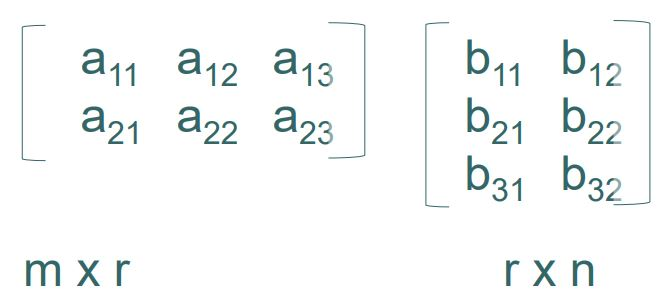
\includegraphics[width=8cm, height=4cm]{1.jpg}
\end{center}
\tab Numărul de operații necesar pentru înmulțirea $A\times B$ este $m\times n\times (2r-1)$. Pentru ușurința calculului, presupunem că folosim întotdeauna matrice pătratice de ordin n, astfel încât calculul devine $2n^3-n^2=O(n^3)$.
\\
\tab Algortmul secvențial este prezentat în cele ce urmează, ideea lui fiind ușor de urmărit. 
\begin{center}
	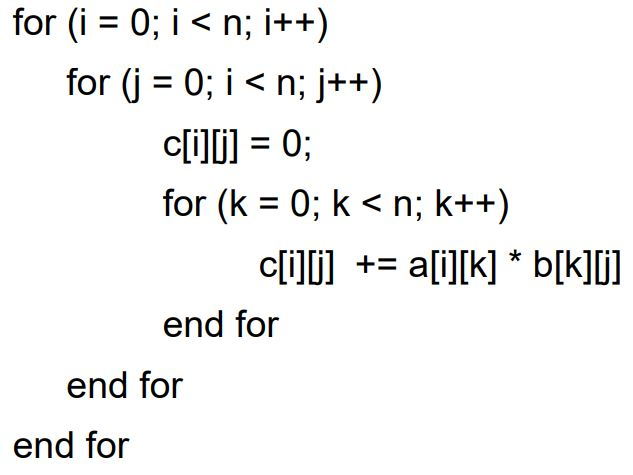
\includegraphics[width=7.5cm, height=5.2cm]{2.jpg}
\end{center}
\tab Vom exemplifica metoda programării paralele pentru înmulțirea a două matrice. Considerăm faptul că cele două matrice au dimensiunea $m\times r$, respectiv $r\times n$. Numărul de procese disponibil este p, matricele înmulțite vor fi A și B, iar rezultatul va fi reprezentat de matricea C. 
\\ 
\tab Implementarea algoritmului: Considerăm cele două matrice A($m\times r$) și B($r\times n$)  care urmează a fi înmulțite.
\begin{enumerate}
  \item Se împarte matricea A în p blocuri pătratice, unde p = numărul de procese disponibile.
  \item Fiecare bloc din A, alături de matricea B sunt trimise către un anumit proces și se calculează înmulțirea acestora, rezultat care este transmis ulterior ca sub-bloc pentru matricea rezultată C.
\end{enumerate}
\tab Procedeul este prezentat în cele ce urmează.
\\ 
\tab 1. Procesul Master trimite către procesele Worker sau Slave rânduri din matricea A, alături de matricea B:
\begin{center}
	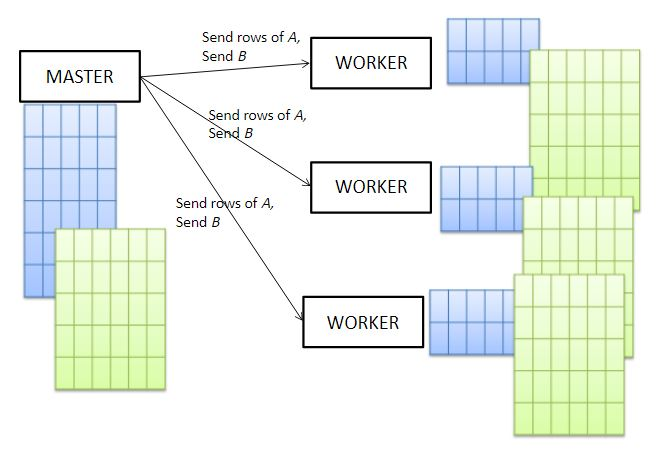
\includegraphics[width=16cm, height=11cm]{3.jpg}
\end{center}
\tab 2. Procesele Worker sau Slave primesc rândurile matricei A corespunzătoare procesului respectiv și întreaga matrice B.
\begin{center}
	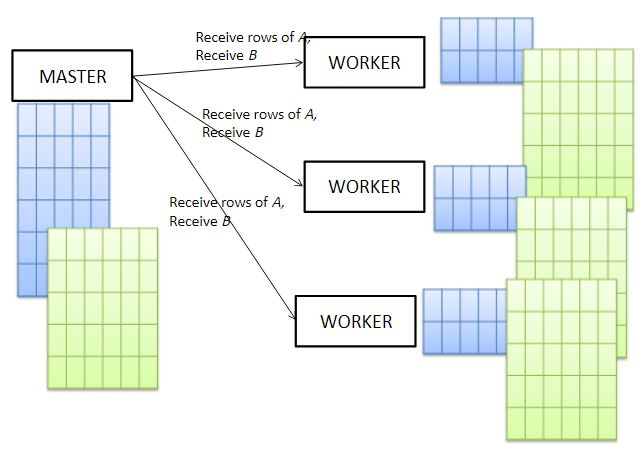
\includegraphics[width=16cm, height=11cm]{4.jpg}
\end{center}
\tab 3. Procesele Worker realizează înmulțirea matricelor primite de către acestea și trimit rezultatul sub formă de bloc procesului Master.
\begin{center}
	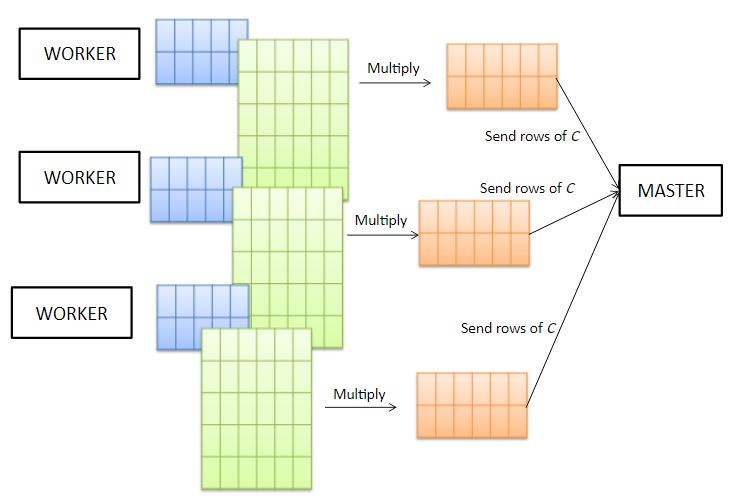
\includegraphics[width=16cm, height=11cm]{5.jpg}
\end{center}
\tab 4. Procesul Master primește blocurile calculate de către procesele Worker și compune rezultatul final, reprezentat de matricea C.
\begin{center}
	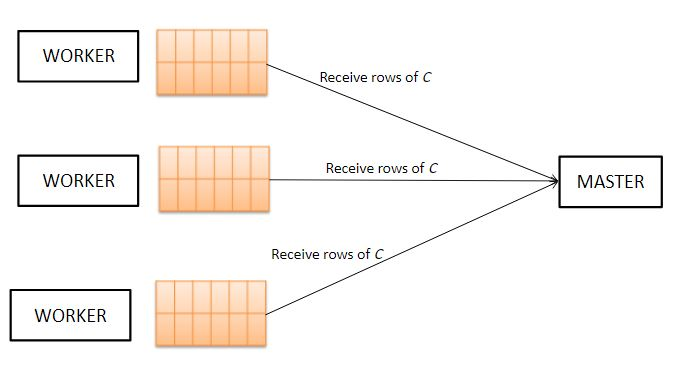
\includegraphics[width=16cm, height=9.5cm]{6.jpg}
\end{center}
\vspace {3cm}
\end{document}


















